\documentclass{article}\usepackage[]{graphicx}\usepackage[]{color}
%% maxwidth is the original width if it is less than linewidth
%% otherwise use linewidth (to make sure the graphics do not exceed the margin)
\makeatletter
\def\maxwidth{ %
  \ifdim\Gin@nat@width>\linewidth
    \linewidth
  \else
    \Gin@nat@width
  \fi
}
\makeatother

\definecolor{fgcolor}{rgb}{0.345, 0.345, 0.345}
\newcommand{\hlnum}[1]{\textcolor[rgb]{0.686,0.059,0.569}{#1}}%
\newcommand{\hlstr}[1]{\textcolor[rgb]{0.192,0.494,0.8}{#1}}%
\newcommand{\hlcom}[1]{\textcolor[rgb]{0.678,0.584,0.686}{\textit{#1}}}%
\newcommand{\hlopt}[1]{\textcolor[rgb]{0,0,0}{#1}}%
\newcommand{\hlstd}[1]{\textcolor[rgb]{0.345,0.345,0.345}{#1}}%
\newcommand{\hlkwa}[1]{\textcolor[rgb]{0.161,0.373,0.58}{\textbf{#1}}}%
\newcommand{\hlkwb}[1]{\textcolor[rgb]{0.69,0.353,0.396}{#1}}%
\newcommand{\hlkwc}[1]{\textcolor[rgb]{0.333,0.667,0.333}{#1}}%
\newcommand{\hlkwd}[1]{\textcolor[rgb]{0.737,0.353,0.396}{\textbf{#1}}}%
\let\hlipl\hlkwb

\usepackage{framed}
\makeatletter
\newenvironment{kframe}{%
 \def\at@end@of@kframe{}%
 \ifinner\ifhmode%
  \def\at@end@of@kframe{\end{minipage}}%
  \begin{minipage}{\columnwidth}%
 \fi\fi%
 \def\FrameCommand##1{\hskip\@totalleftmargin \hskip-\fboxsep
 \colorbox{shadecolor}{##1}\hskip-\fboxsep
     % There is no \\@totalrightmargin, so:
     \hskip-\linewidth \hskip-\@totalleftmargin \hskip\columnwidth}%
 \MakeFramed {\advance\hsize-\width
   \@totalleftmargin\z@ \linewidth\hsize
   \@setminipage}}%
 {\par\unskip\endMakeFramed%
 \at@end@of@kframe}
\makeatother

\definecolor{shadecolor}{rgb}{.97, .97, .97}
\definecolor{messagecolor}{rgb}{0, 0, 0}
\definecolor{warningcolor}{rgb}{1, 0, 1}
\definecolor{errorcolor}{rgb}{1, 0, 0}
\newenvironment{knitrout}{}{} % an empty environment to be redefined in TeX

\usepackage{alltt}

\usepackage[backend=bibtex, sorting=none, citestyle=authoryear]{biblatex}

\bibliography{references}


\title{Efficiency}
\author{Aidan Morrison}
\IfFileExists{upquote.sty}{\usepackage{upquote}}{}
\begin{document}

\maketitle




\section{Introduction}

\subsection{Another Idea}

The purpose of this paper is to investigate the suitability of the pump-jet selection for Australia's future fleet of submarines.  In particular, the question of the relative efficiency, and quietness of pump-jets in comparison to open propellers is of particular importance.  Much has been made of the significance of the pump-jet in the DCNS (now Naval Group) bid for the submarine, to the extent that it has been claimed that the pump-jet rendered propellers obsolete.

Necessarily, this topic depends upon a considerable amount of physics, particularly around hydrodynamics, fluid mechanics, and turbomachinery, all of which might be difficult or daunting topics to usefully inform a public policy debate. However, in the case of a \$50 billion dollar military acquisition, neglecting to engage with the technical matters that are so crucial to such a decision would be deeply foolish.  To that end, this paper has a very specific ambition.  It doesn't seek to advance the technical field with any new research or insight.  Instead, it aims to make as much of the relvant physics as possible to this particular question comprehensible in laymans terms, and connect the essential concepts as directly as possible with the most important conclusions of public import.


\section{Executive Summary}

\subsection{The difference between nuclear and conventional for speed}

This paper was commissioned in order to investigate whether pumpjets could plausibly be as efficient, or more efficient than a suitably designed open propeller for a conventional submarine. A crucial input to the investigation is a rough understanding of what the speeds of operation are likely to be for a submarine.  Whereas nuclear submarines are reportedly capable of reaching speeds in excess of 30kt, and might transit long distances at such high speeds, conventional sumbarines are not thought of as being able to reach speeds far above 20kt in a sprint, and can only sustain speeds of 8-10kt for long-distance transits.  Moreover, on patrol, a large portion of thier work is done at very low speeds, typically thought to be in the range of 2-4kt. 


\subsection{The importance of low speed operation for diesel-electric submarines}

The efficiency of the propulsion system at such low speeds is of great significance for a conventional submarine, since it must rely on batteries or other air-independent propulsion sources for power when entirely submerged.  Consequently, excessive energy consumption results in greatly reduced dived endurances.  Since a submarine's position is vastly more likely to be discovered when it is on the surface operating its diesel engines, this ability to remain submerged for a long time is crucially important for combat operations, and in transiting through sensitive or contested areas.  For nuclear submarines, which posess a practically infinite supply of energy from the nuclear reactor, efficiency at low speeds is of no concern.  In fact, dispersing additional energy, (provided it can be done quietly) is probably advantageous for a nuclear submarine, since it will allow the nuclear reactor to avoid running at very low power levels, where the stability of the reactor is reduced.

\subsection{The necessity of drag, and decelleration, induced by the duct}

The role of the shroud (or tunnel, mantel, duct) around the jet is to allow the pressure to be raised around the impeller, in a way that is not possible for an open propeller.  By a fundamental requirements of physics, this actually requires that the water's incoming speed be \textbf{reduced} before it reaches the impeller. (The kinetic energy embodied in movement is converted into potential energy, or pressure.)  Whilst the duct narrowing at the nozzle also necessarily accelerates the water, (as the additinal pressure imparted by the impeller is converted back to kinetic energy) it's an essential feature of all pump-jets that the water flow is decelerated at the point of reaching the impeller. Consequently, an elementary form of the pump-jet is also termed the 'decelerating duct' applied to a propeller.  Put simply, the water has to slow down to go fast again.


\section{Speed and Drag - Why very slow is very very $(very)^2$ economical}

Perhaps the most important relationship to understand is the relationship between speed and drag as it pertains to submarines.  This is immportant because it sets out the fundamental framework as it applies to any submarine, regardless of propulsion type.  (It's also a pretty important for planes, cars, missiles, torpedoes, and basically everything else.)

Drag is the resistance that a fluid (air or water, in our case) gives to a body that is passing through it. Quite simply, it's a force that acts in the opposite direction.  There are multiple sources of drag for different types of scenarios.  For scenarios where an object is in contact with two different types of fluid (like a ship, on the ocean) or when the fluid doesn't really have contact with all of the object (supersonic flight, and supercavitating torpedoes) some more complex physics applies. For a fuller discussion of types of drag, see \parencite{carlton2007}. But in the case of a submarine, which does it's business completely immersed in the ocean, the relevant physics is dominated the skin friction on the hull, which follows a very simple rule and relationship.  The amount of drag ($F_D$) an objet experiences increases directly in proportion to the surface area $A$.  For any given object of a certain (unchanging shape) there will be a constant coefficent ($C_D$) which reflects how aerodynamic or hydrodymanic the shape is.  The drag is also directly proportional to the density of the fluid being moved through, $\rho$.  (Air creates roughly one-thousandth the drag as water does on any given object at a given speed, since it's roughly one thousand times less dense.)


\begin{equation} 
\label{eq:1}
F_D = \frac{1}{2}\rho v^2C_DA
\end{equation}

\footnote{Technical aside: This law applies wherever the the flow over the surface is turbulent. It is true that for very small objects, or very viscous fluids, or very slow movements a different apples called Stokes Equation, in the case wher Reynolds numbers are less than 1.  Given that sea-water is not particularly viscous, and sumbarines not particularly small, Reynolds numbers are liekly to be much much greater than 1 (one or two thousand), even when moving at only one or two knots.  Since it is unlikely that a significant proportion of the flow over the hull will be laminar, we'll use the drag equation in all modeling going forward when considering drag on the hull.}

It's crucial to understand, however, that drag is only a force, and doesn't directly inform us about how much energy is consumed, until we multiply it by the **distance** over which it is applied, not the time for which it is applied.  To think about it simply, gravity exerts a force on you downwards all the time.  But you don't expend any energy overcoming it when sitting still.  If you climb stairs, the amount of gravitational potential you attain depends on how high up you climb, not how long you spend on the ladder or stair-case.




\section{The difference between nuclear and conventional propulsion}

Nuclear submarines vary quite remarkably from conventional submarines because of the means by which they generate their power.  Because of the extremely high energy density in enriched uranium or plutonium, the reactors on board nuclear submarines generate an abundant supply of energy.  Most submarine reactors are reportedly capable of generating between 25 to 50 megawatts (MW) of power, though Russian submarines have hundreds of megawatts of power available \parencite{WNA2017}.

In contrast, the Collins Class Submarine's main motor is rated at less than 6MW, with designs for the future submarine appearing to be only slightly larger \parencite{patrick2012}.  It is fair to say that in terms of maximum power ouput, nuclear submarines could have something like 5-10 times as much power at their disposal, and their \textbf{peak} output.  

The difference between the peak-powers of the submarines significantly understates how different the designs are, because the difference in the total amount of energy stored and available for use in a voyage or dive is vastly greater.  A nuclear submarine might have literally millions of times more energy at its disposal, it is practically unlimited for all intents and purposes on a given voyage. Consequently, wheras a nuclear submarine might regularly conduct transits at or near it's peak power, a diesel electric submarine would probably transit at less than half the speed which it could manage at a sprint, (and use less than a quarter of the energy, as discussed earlier) and on patrol it might be operating at a tenth of the maximum speed, and use maybe just 1\% of as much power on propulsion. In this situation, the amount of power that is drawn for lights, CO2 scrubbing, washing, cooking, heating, as well as the electronics driving the combat systems (the 'Hotel Load') might well become significant, and even be as larger or larger than what is required for propulsion.

Consequently, the difference between the power output a conventional and a nuclear submarine might regularly operate at could be even quite a bit larger than the maximum amount of energy that they can deliver to their propulsion systems.  

Perhaps more significantly for power-design of nuclear submarines is a little-discussed phenomenon called Xenon poisoning, which affects nuclear reactors when they shut down or lower their power significantly. When Uranium or Plutonium atoms split (or fission) into two smaller isotopes atoms, a variety of different radio nucleides (unstable variants of atoms) are produced.  Two of these are Xenon-135 and Iodine 135.  Iodine is produced much more often, and decays into Xenon-135, which a half-life of about nine hours.  This Xenon has a very special, perhaps unique role in reactors, since they very easily captures the free neutrons which cause the continued fission reactions in Uranium or Plutonium which drive the reactor.  As such, Xenon is known as reactor 'poison' since it can kill the reactor's reactivity in very high doses.

This high neutron-capture from Xenon means that it has a duplicitous relationship with the reactor's power level.  At high levels of reactor power, lots of Xenon-135 and Iodine-135 are produced by the fission process.  The high presence of Xenon reduced the reactor's reactivity.  On the other hand, there are lots of neutrons available to 'burn off' the ass Xenon (which absobs the neturons to become a different isotope).  This keeps the total level of Xenon in check.  

The situation becomes much more complicated when the reactor undergoes a sudden change in power output.  If the power is lowered dramatically and suddenly, the production of Xenon continues quite rapidly for some time due to the decay of the large stock of Iodine-135.  With less neutron flux available to 'burn off' the Xenon, the Xenon levels spike, and push down the reactor's reactivity.  Unless the reactor is quickly raised back to relatively high power (~60\%) quite quickly (an hour or less), the Xenon levels become so high that the reactor will have to be shut down, otherwise extreme (and dangerous) measures would be required in order to keep the reactor going.  (This is essentially what lead to the Chernobyl Explosion \parencite{WNA2009}.)  A fuller discussion of Xenon poisoning can be found in \citetitle{garland2005}  by \citeauthor{garland2005}, which demonstrates key concepts related to the poisoning effect shown in Figure \ref{fig:xenon}.

The situation becomes much more complicated when the reactor undergoes a sudden change in power output.  

\begin{figure}
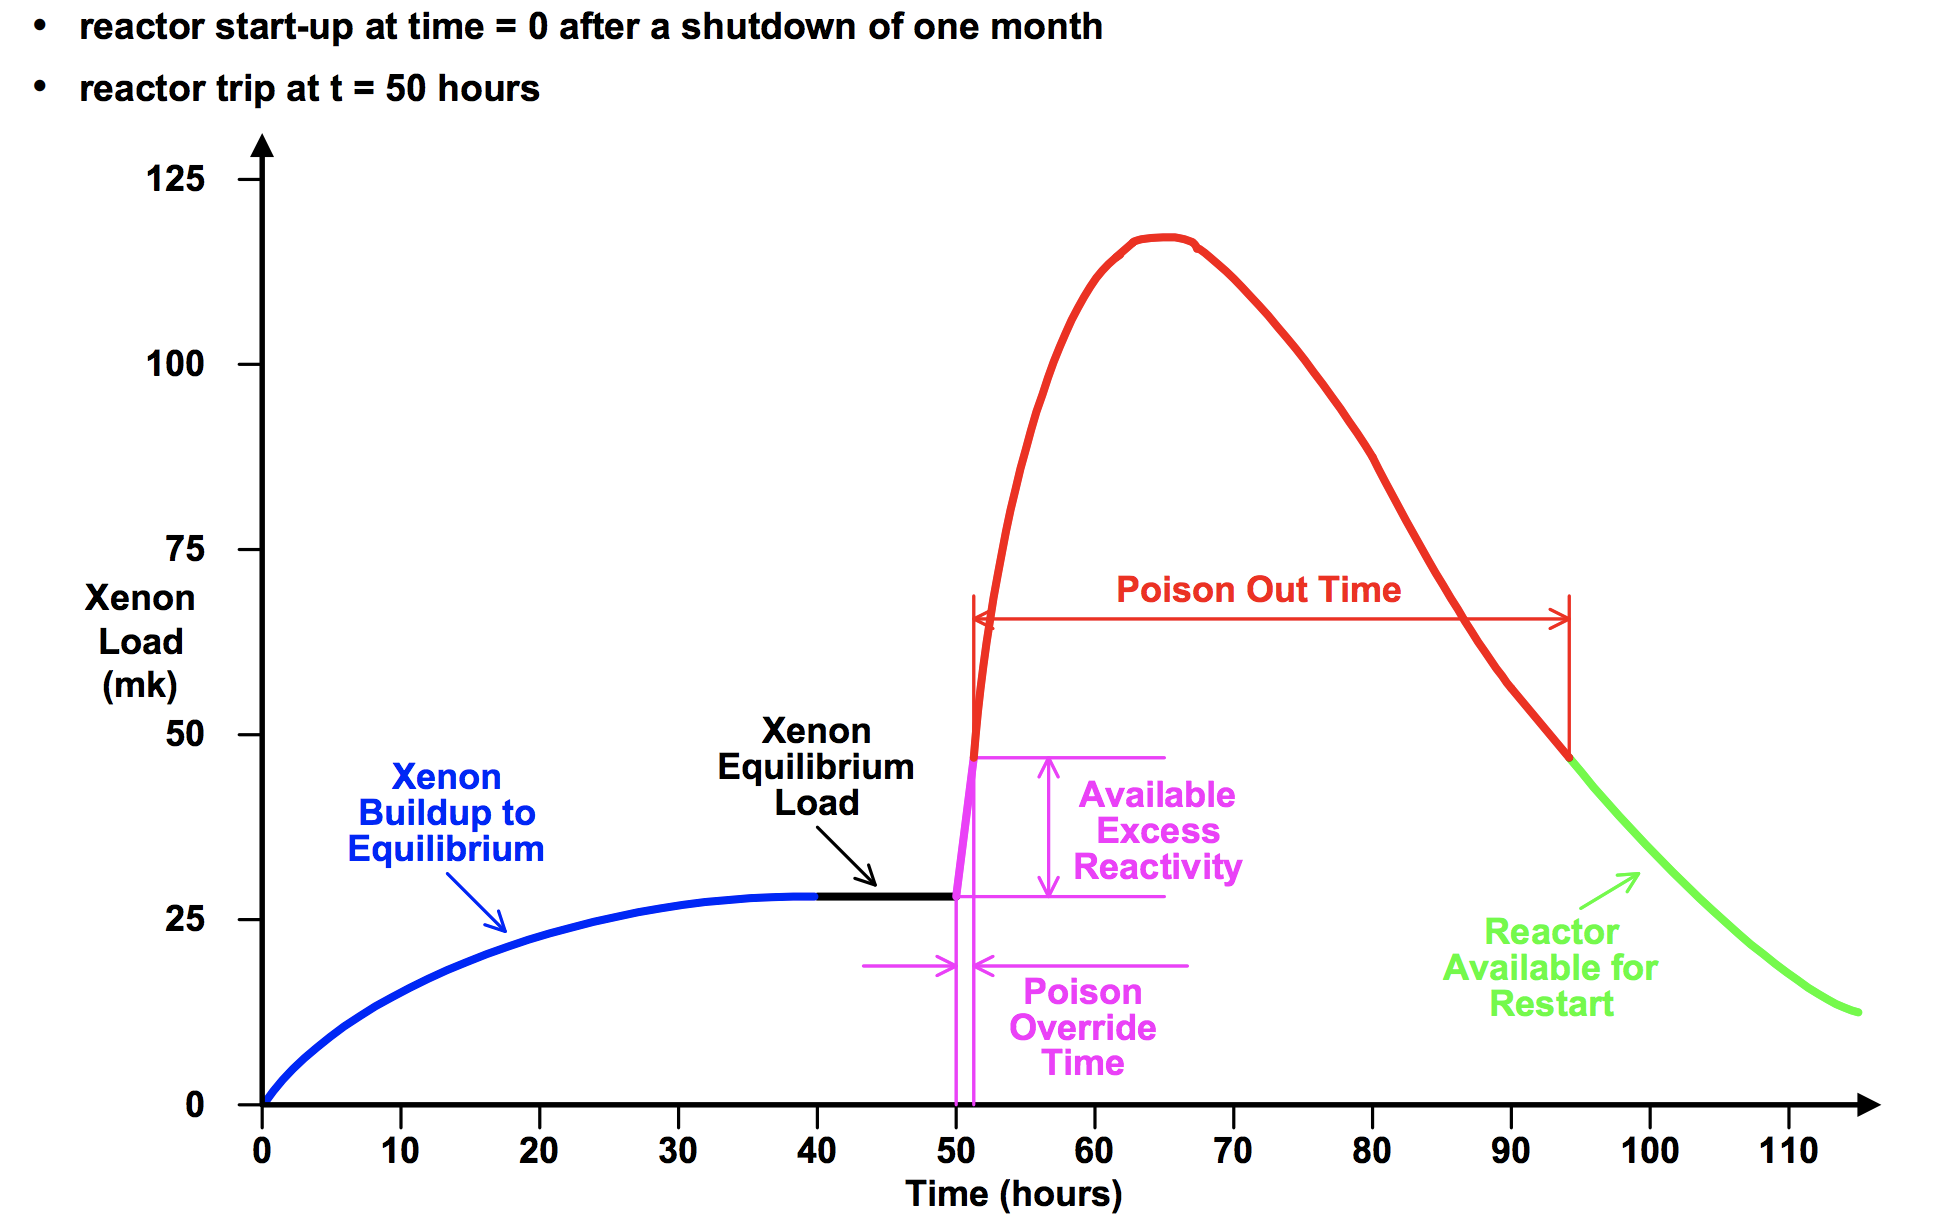
\includegraphics[width=0.9\textwidth]{XenonPoison.png}
\caption{A prototype of the Job Information dialog \parencite{garland2005}}
\label{fig:xenon}
\end{figure}

In Figure \ref{fig:ex2} we can see a sample plot of the mtcars data.

\begin{figure}
\begin{knitrout}
\definecolor{shadecolor}{rgb}{0.969, 0.969, 0.969}\color{fgcolor}

{\centering 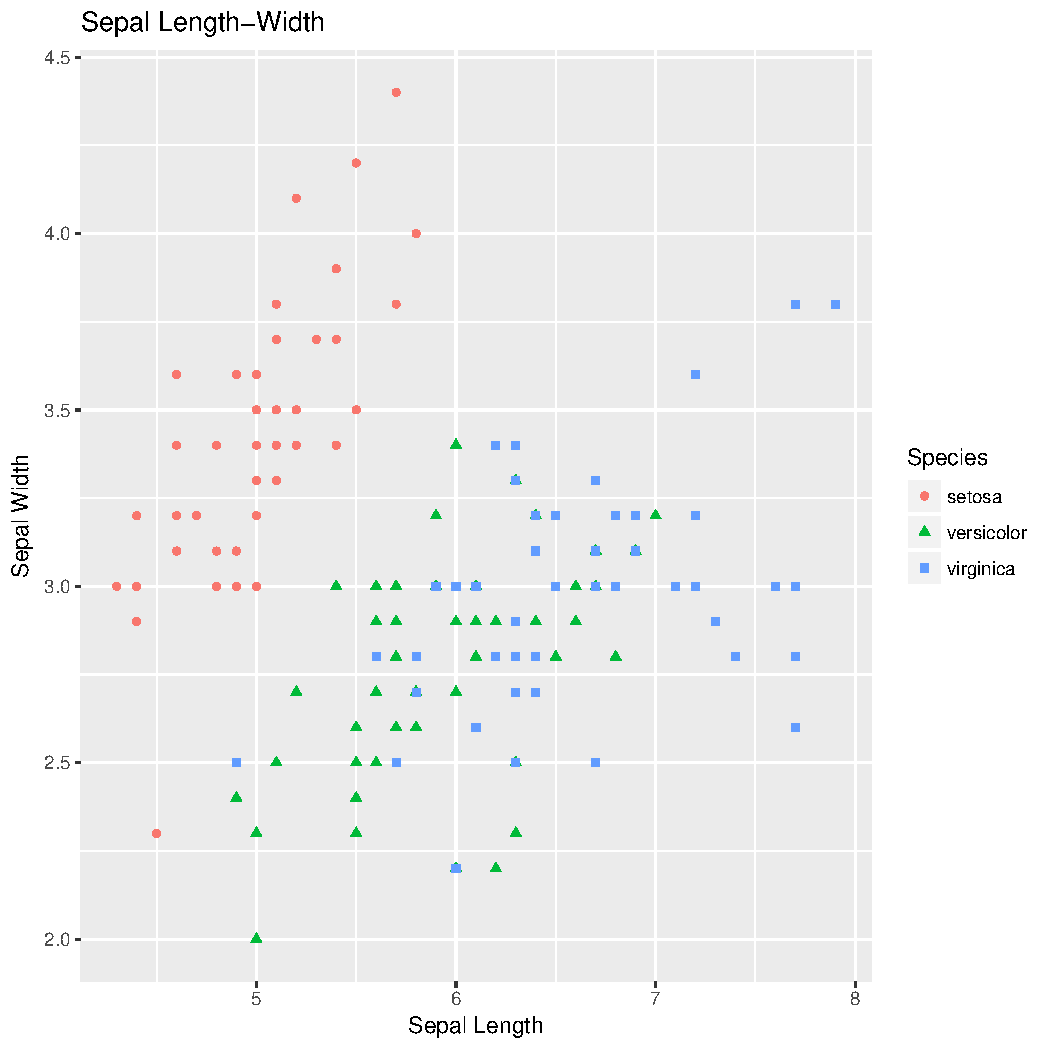
\includegraphics[width=\maxwidth]{figures/plots-unnamed-chunk-1-1} 

}



\end{knitrout}
\caption{An example plot}
\label{fig:ex2}
\end{figure}
 

Consequently, nuclear reactors aren't well suited to rapid fluctuations in power, particularly dramatic reductions in power, as these can lead to instability in the reactor core.  If the reactor is shut down in order to avoid such dangerous circumstances, it generally cannot be started again until Xenon levels have fallen again, which can take a couple of days.  Obviously this is never desirable for a military vessel, and hence is avoided at almost all costs. 

 
This effect has a dramatic impact on nuclear submarine design, since much of their design is oriented around being able to comfortably disperse large amounts of excess power, rather than with conserving it.  For the propulsion system, this actually makes having an inefficient propulsor at low speeds a considerable advantage.  Since the reactor will likely need to dispose of excess power, particularly during ramp-down, an inefficient propulsion system actually provides a useful power sink.  Since any excess power will have to be disposed of by some other means (normally by pumping more water to remove the power as the heat) inefficiency at low speeds has no penalty, and probably a marginal benefit, since it will reduce overall demand for additional systems.    Provided the excess turbulence inside the pumpjet isn't too noisy, wasting energy through the propulsor is useful. 


It should also be noted that a nuclear reactor's aversion to sudden reductions in power would also have a substantial impact on the design of a submarine's combat system, and it's demand on the Hotel Load. For the same reason, a high Hotel Load, or power-hungry Combat System, could actually be advantageous, as it helps to set an elevated 'floor' for power requirements, reducing the scale of fluctuations in overall power demand from the reactor due to changes in propulsion speed.  


\printbibliography
 
\end{document}
